\datos{color}{}{}

\subsection{\textit{TIAGo}}

\textit{TIAGo} (acrónimo de \textit{Take It And Go}), Figura \ref{tiago}, es un robot colaborativo móvil desarrollado por 
\textit{PAL Robotics}, empresa con sede en Barcelona especializada 
en robótica de servicio y plataformas colaborativas, a partir de 2015 y ampliamente utilizado en investigación en robótica de 
servicio, interacción humano–robot y manipulación autónoma. Combina una base móvil diferencial u omnidireccional, 
uno o dos brazos manipuladores colaborativos de 7 grados de libertad cada uno y un torso elevable, lo que le permite 
realizar tareas complejas de navegación y manipulación en entornos humanos. \\

Sus usos principales incluyen la asistencia en entornos domésticos y hospitalarios, la 
manipulación colaborativa, la navegación autónoma en interiores, la investigación en 
interacción humano–robot, la percepción avanzada y la participación en competiciones 
robóticas como la \textit{RoboCup@Home}. Su versatilidad lo convierte en una plataforma 
estándar en numerosos laboratorios europeos. \\

\begin{wrapfigure}{r}{0.5\textwidth}
    \centering
    \vspace{-10pt}
    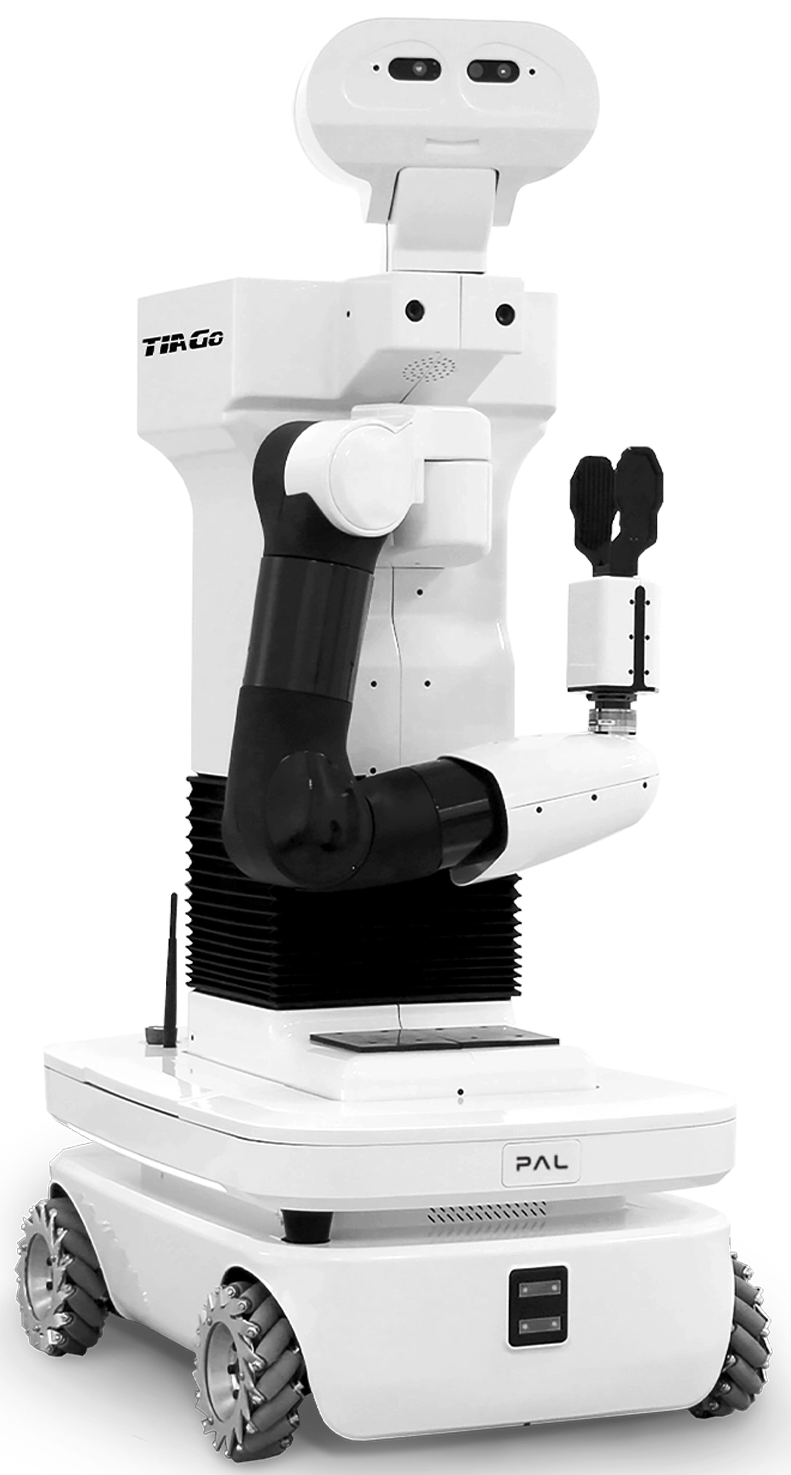
\includegraphics[width=0.2\textwidth]{Images/tiago.png}
    \caption{\textit{TIAGo}.}
    \label{tiago}
    \vspace{-10pt}
\end{wrapfigure}

La arquitectura del sistema es híbrida, combinando control centralizado para la planificación 
global y módulos distribuidos para la percepción, la navegación y el control del manipulador. 
El robot integra un ordenador embarcado de alto rendimiento que ejecuta \textit{ROS2} y gestiona 
la fusión sensorial, \textit{SLAM}, la planificación de trayectorias y la supervisión del sistema. 
Los controladores de bajo nivel del brazo, la base y el torso funcionan como nodos 
independientes, comunicándose mediante ROS2 y buses internos en tiempo real. \\

El método de locomoción se basa en una base móvil con ruedas diferenciales u omnidireccionales 
(según la configuración), equipada con sensores láser \textit{2D/3D}, cámaras \textit{RGB-D} y 
odometría. Esta base permite navegación autónoma, evitación de obstáculos y movimientos 
precisos en espacios estrechos. Los manipuladores colaborativos de 7 grados de libertad, 
accionados por motores eléctricos y 
reductores armónicos, permiten realizar tareas de manipulación segura junto a humanos.

\subsection*{Referencias}

\cite{Pags2016TIAGoTM} \fullcite{Pags2016TIAGoTM}.\\
\cite{TiagoRef} \fullcite{TiagoRef}.
